%----------------------- Преамбула -----------------------
\documentclass[ut8x, 14pt, oneside, a4paper]{extarticle}
\usepackage{extsizes} % Для добавления в параметры класса документа 14pt

% Для работы с несколькими языками и шрифтом Times New Roman по-умолчанию
\usepackage[english,russian]{babel}
\usepackage{fontspec}
\setmainfont{Times New Roman}
\usepackage[left=30mm,right=10mm,top=20mm,bottom=20mm]{geometry}
\usepackage{misccorr}
\usepackage{indentfirst}
\usepackage{enumitem}
\usepackage{pdfpages}
\usepackage{placeins}
%\usepackage{ragged2e}
\setlength{\parindent}{1.25cm}
%\setlength{\parskip}{1em} % поменять
%\linespread{1.3}
\renewcommand{\baselinestretch}{1.5}
\setlist{nolistsep} % Отсутствие отступов между элементами \enumerate и \itemize

% Дополнительное окружения для подписей
\usepackage{array}
\newenvironment{signstabular}[1][1]{
	\renewcommand*{\arraystretch}{#1}
	\tabular
}{
	\endtabular
}

% Переопределение стандартных \section, \subsection, \subsubsection по ГОСТу;
% Переопределение их отступов до и после для 1.5 интервала во всем документе
\usepackage{titlesec}

\titleformat{\section}[block]
{\bfseries\normalsize\filcenter}{\thesection}{1em}{}

\titleformat{\subsection}[hang]
{\bfseries\normalsize}{\thesubsection}{1em}{}
\titlespacing\subsection{\parindent}{\parskip}{\parskip}

\titleformat{\subsubsection}[hang]
{\bfseries\normalsize}{\thesubsubsection}{1em}{}
\titlespacing\subsubsection{\parindent}{\parskip}{\parskip}

\newcommand{\specsection}[1]{\section*{#1}\addcontentsline{toc}{section}{#1}}
\newcommand{\specsubsection}[1]{\subsection*{#1}\addcontentsline{toc}{subsection}{#1}}
\newcommand{\specsubsubsection}[1]{\subsubsection*{#1}\addcontentsline{toc}{subsubsection}{#1}}

% Работа с изображениями и таблицами; переопределение названий по ГОСТу
\usepackage{caption}
\captionsetup[figure]{name={Рисунок},labelsep=endash}
\captionsetup[table]{singlelinecheck=false, labelsep=endash}

\usepackage{graphicx}
\usepackage{diagbox} % Диагональное разделение первой ячейки в таблицах

% Цвета для гиперссылок и листингов
\usepackage{color}

% Гиперссылки \toc с кликабельностью
\usepackage[linktoc=all]{hyperref}
\hypersetup{hidelinks}

% Листинги
%\setsansfont{Arial}
%\setmonofont{Courier New}

\usepackage{color} % Цвета для гиперссылок и листингов
%\definecolor{comment}{rgb}{0,0.5,0}
%\definecolor{plain}{rgb}{0.2,0.2,0.2}
%\definecolor{string}{rgb}{0.91,0.45,0.32}
%\hypersetup{citecolor=blue}
\hypersetup{citecolor=black}

\newcommand{\anonsection}[1]{%
	\section*{\centering#1}%
	\addcontentsline{toc}{section}{#1}%
}

\usepackage{pgfplots}
\pgfplotsset{width=7cm,compat=1.9}

\usepackage{caption}
\DeclareCaptionFont{white}{\color{white}}
\DeclareCaptionFormat{listing}{\colorbox{white}{\parbox{\textwidth}{#1#2#3}}}
\captionsetup[lstlisting]{format=listing,justification=raggedright}
\usepackage{listings}
\lstset{
	basicstyle=\footnotesize\ttfamily,
	language=C, % Или другой ваш язык -- см. документацию пакета
	numbers=left,
	numbersep=5pt,
	tabsize=2,
	extendedchars=\true,
	breaklines=true,
	keywordstyle=\color{blue},
	frame=single,
	showspaces=false,
	showtabs=false,
	xleftmargin=17pt,
	framexleftmargin=17pt,
	framexrightmargin=-5pt,
	framexbottommargin=4pt,
	showstringspaces=false,
	inputencoding=utf8x,
	keepspaces=true
}

%\DeclareCaptionLabelSeparator{line}{\ --\ }
%\DeclareCaptionFont{white}{\color{white}}
%\DeclareCaptionFormat{listing}{\colorbox[cmyk]{0.43,0.35,0.35,0.01}{\parbox{\textwidth}{\hspace{15pt}#1#2#3}}}
%\captionsetup[lstlisting]{
	%	format=listing,
	%	labelfont=white,
	%	textfont=white,
	%	singlelinecheck=false,
	%	margin=0pt,
	%	font={bf,footnotesize},
	%	labelsep=line
	%}

\usepackage{ulem} % Нормальное нижнее подчеркивание
\usepackage{hhline} % Двойная горизонтальная линия в таблицах
\usepackage[figure,table]{totalcount} % Подсчет изображений, таблиц
\usepackage{rotating} % Поворот изображения вместе с названием
\usepackage{lastpage} % Для подсчета числа страниц

\makeatletter
\renewcommand\@biblabel[1]{#1.}
\makeatother

\usepackage{color}
\usepackage[cache=false, newfloat]{minted}
\newenvironment{code}{\captionsetup{type=listing}}{}
\SetupFloatingEnvironment{listing}{name=Листинг}

\usepackage{amsmath}
\usetikzlibrary{datavisualization}
\usetikzlibrary{datavisualization.formats.functions}
\usepackage{csvsimple}

% !TeX TXS-program:compile = txs:///lualatex/[--shell-escape]

\begin{document}
	\begin{titlepage}
		\noindent\begin{minipage}{0.05\textwidth}
			
\includegraphics[scale=0.3]{inc/bmstu.png}
		\end{minipage}
		\hfill
		\begin{minipage}{0.85\textwidth}\raggedleft
			\begin{center}
				\fontsize{12pt}{0.3\baselineskip}\selectfont \textbf{Министерство науки и высшего образования Российской Федерации \\ Федеральное государственное бюджетное образовательное учреждение \\ высшего образования \\ <<Московский государственный технический университет \\ имени Н.Э. Баумана \\ (национальный исследовательский университет)>> \\ (МГТУ им. Н.Э. Баумана)}
			\end{center}
		\end{minipage}
		
		\begin{center}
			\fontsize{12pt}{0.1\baselineskip}\selectfont
			\noindent\makebox[\linewidth]{\rule{\textwidth}{4pt}} \makebox[\linewidth]{\rule{\textwidth}{1pt}}
		\end{center}
		
		\begin{flushleft}
			\fontsize{12pt}{0.8\baselineskip}\selectfont 
			
			ФАКУЛЬТЕТ \uline{<<Информатика и системы управления>> \hfill}
			
			КАФЕДРА \uline{\mbox{\hspace{4mm}} <<Программное обеспечение ЭВМ и информационные технологии>> \hfill}
		\end{flushleft}
		
		\vfill
		
		\begin{center}
			\fontsize{20pt}{\baselineskip}\selectfont
			
			\textbf{РАСЧЕТНО-ПОЯСНИТЕЛЬНАЯ ЗАПИСКА}
			
			\textit{К КУРСОВОЙ РАБОТЕ}
			
			\textit{НА ТЕМУ:}
		\end{center}
		
		\begin{center}
			\fontsize{18pt}{0.6cm}\selectfont 
			
			<<Разработка загружаемого модуля ядра Linux для мониторинга использования оперативной памяти>>
			
		\end{center}
		
		\vfill
		
		\begin{table}[h!]
			\fontsize{12pt}{0.7\baselineskip}\selectfont
			
			\begin{signstabular}[0.55]{p{7.25cm} >{\centering\arraybackslash}p{4cm} >{\centering\arraybackslash}p{4cm}}
				Студент \uline{~~ИУ7-76Б~~} & \uline{\mbox{\hspace*{4cm}}} & \uline{\hfill А. А. Петрова \hfill} \\
				\scriptsize \hspace*{2cm}(Группа)	& \scriptsize (Подпись, дата) & \scriptsize (И.О. Фамилия)
			\end{signstabular}
			
			\vspace{\baselineskip}
			
			\begin{signstabular}[0.55]{p{7.25cm} >{\centering\arraybackslash}p{4cm} >{\centering\arraybackslash}p{4cm}}
				Руководитель & \uline{\mbox{\hspace*{4cm}}} & \uline{\hfill Н. Ю. Рязанова \hfill} \\
				& \scriptsize (Подпись, дата) & \scriptsize (И.О. Фамилия)
			\end{signstabular}
		\end{table}
		
		\vfill
		
		\begin{center}
			\normalsize \textit{2023 г.}
		\end{center}
	\end{titlepage}

\pagenumbering{gobble}
%\include{tex/tz.tex}
\normalsize
\pagenumbering{arabic}
\setcounter{page}{2}

%\section*{РЕФЕРАТ}

Расчетно-пояснительная записка 36 с., 10 рис., 5 табл., 7 ист., 5 прил.

Объектом разработки в данной работе является база данных, содержащая информацию о репетиционных базах, соответствующих им комнатах и оборудовании, с целью предоставить возможность пользователям искать необходимые комнаты и бронировать свои репетиции. Цель данной работы – реализовать приложение, содержащее информацию о репетиционных базах. В приложении, работающем с этой БД, должна быть возможность для музыканта бронировать или отменять свои репетиции, а для владельца реп. базы - отслеживать записи на свою реп. базу.

Чтобы достигнуть поставленной цели, требуется решить следующие задачи:
\begin{itemize}
	\item формализовать задание, определить необходимый функционал;
	\item провести анализ СУБД;
	\item описать структуру БД;
	\item создать и заполнить БД;
	\item разработать ПО, которое позволит пользователю-музыканту бронировать и отменять свои репетиции, а владельцу отслеживать их;
	\item провести исследование зависимости времени выполнения запроса от числа записей в таблице.
\end{itemize}

Поставленная цель достигнута: в ходе курсового проекта была разработана база данных, хранящая информацию о репетиционных точках. При этом при разработке в качестве СУБД использовался PostgreSQL, а в качестве языка программирования – Python 3.7.

Дальнейшее развитие проекта подразумевает:
\begin{itemize}
	\item добавление фотографий комнат в блок информации о них;
	\item добавление календаря для более удобного бронирования репетиций;
	\item добавление возможности бронировать не только репетиционные базы, но и другие творческие площадки;
	\item добавление возможности администраторам блокировать пользователей;
	\item создание мобильной версии приложения.
\end{itemize}

КЛЮЧЕВЫЕ СЛОВА

\textit{базы данных, разработка ПО, репетиционные базы, бронирование репетиций, postgresql, python.}

\clearpage

\renewcommand{\contentsname}{\normalsize\bfseries\centering СОДЕРЖАНИЕ}
\tableofcontents
\clearpage


\specsection{Введение}

В настоящее время большую актуальность имеют системы, предоставляющие информацию о ресурсах операционной системы и частоте системных вызовов. Имея такие сведения, пользователь может проанализировать состояние системы и нагрузку на неё. Особое внимание уделяется операционным системам с ядром Linux~\cite{linux}. Ядро Linux возможно изучать благодаря тому, что оно имеет открытый исходный код.

На данный момент существует множество различных утилит и команд для получения информации о свободной и занятой оперативной памяти в Linux. Одни из наиболее известных -- это команды free, vmstat, htop, memstat~\cite{commands}. Также существует приложение GNOME System Monitor, предоставляющее краткую статистику использования системных ресурсов -- памяти, процессора, подкачки и сети -- в графическом виде~\cite{gnome}.
\section{Аналитическая часть}

\subsection{Постановка задачи}

В соответствии с заданием необходимо разработать загружаемый модуль ядра, предоставляющий статистику по количеству доступной и занятой оперативной памяти за выбранный промежуток времени.

Требования к разрабатываемому ПО:
\begin{itemize}
	\item ПО должно выдавать количество свободной, доступной и занятой оперативной памяти каждые 10 секунд;
	
	\item полученная информация должна записываться в виртуальную файловую систему /proc в файл /proc/monitor/memory.
\end{itemize}

Ограничения на разрабатываемое ПО:
\begin{itemize}
	\item ПО не предоставляет информацию о том, чем конкретно занята оперативная память;
	
	\item промежуток времени задается внутри программы и может быть изменен только в коде.
\end{itemize}

\subsection{Основные понятия}

\textbf{Свободная память} -- память, которая в настоящее время ни для чего не используется~\cite{freemem}.

\textbf{Доступная память} -- память, которая используется, но может быть предоставлена для новых или существующих процессов.

\textbf{Занятая память} -- память, которая на данный момент уже используется процессами.

\textbf{Нижняя область памяти} -- область, к которой ядро может обращаться напрямую. Все структуры данных ядра находятся в этой области.

\textbf{Верхняя область памяти} -- область, доступ к которой осуществляется через косвенные механизмы. Здесь находится кэш данных.

\subsection{Анализ методов решения}

\subsubsection{Файл /proc/meminfo}

Одним из способов получения информации об использовании памяти является файл /proc/meminfo~\cite{meminfo}. Из /proc/meminfo можно получить информацию о свободной памяти, об используемой (и физической, и swap), а также о разделяемой (shared memory) и буферах.

Основные показатели:

\begin{itemize}
	\item MemTotal -- общий объем оперативной памяти;
	
	\item LowFree -- объем свободной нижней области памяти;
	
	\item HighFree -- объем свободной верхней области памяти;
	
	\item MemFree -- сумма LowFree и HighFree;
	
	\item MemAvailable -- объем доступной оперативной памяти.
\end{itemize}

Помимо перечисленных в /proc/meminfo присутствует также множество других показателей, не существенных для данной работы.

Основной недостаток использования такого метода решения поставленной задачи заключается в необходимости постоянного обращения напрямую к указанному файлу и его анализа, что может привести к дополнительным временным затратам.

\subsubsection{Структура struct sysinfo}

Чтобы избежать чтения и анализа упомянутого выше файла, можно использовать структуру struct sysinfo.

Структура struct sysinfo~\cite{sysinfo} хранит статистику о всей системе: информацию о времени, прошедшем с начала запуска системы, количество занятой памяти и так далее. В листинге~\ref{lst:sysinfo} приведено объявление рассматриваемой структуры.

\begin{lstlisting}[label={lst:sysinfo}, caption={структура struct sysinfo}]
	struct sysinfo {
		__kernel_long_t uptime;		/* Seconds since boot */
		__kernel_ulong_t loads[3];	/* 1, 5, and 15 minute load averages */
		__kernel_ulong_t totalram;	/* Total usable main memory size */
		__kernel_ulong_t freeram;	/* Free memory size */
		__kernel_ulong_t sharedram;	/* Amount of shared memory */
		__kernel_ulong_t bufferram;	/* Memory used by buffers */
		__kernel_ulong_t totalswap;	/* Total swap space size */
		__kernel_ulong_t freeswap;	/* swap space still available */
		__u16 procs;		   	/* Number of current processes */
		__u16 pad;		   	/* Explicit padding for m68k */
		__kernel_ulong_t totalhigh;	/* Total high memory size */
		__kernel_ulong_t freehigh;	/* Available high memory size */
		__u32 mem_unit;			/* Memory unit size in bytes */
		char _f[20-2*sizeof(__kernel_ulong_t)-sizeof(__u32)];	/* Padding: libc5 uses this.. */
	};
\end{lstlisting}

Для инициализации этой структуры используется функция si\_meminfo(). Стоит отметить, что рассматриваемая структура не содержит информации о доступной памяти в системе. Для того чтобы получить эту информацию, необходимо воспользоваться функцией si\_mem\_available().

\subsection{Загружаемые модули ядра}

Одной из особенностей ядра Linux является способность расширения функциональности во время работы, без необходимости компиляции ядра заново. Часть кода, которая может быть добавлена в ядро во время работы, называется \textbf{модулем ядра}. Ядро Linux предлагает поддержку большого числа классов модулей. Каждый модуль -- это подготовленный объектный код, который может быть загружен в работающее ядро, а позднее может быть выгружен из ядра. Чтобы загрузить модуль в ядро, необходимо воспользоваться командой <<insmod name.ko>>. А для выгрузки модуля -- командой <<rmmod name.ko>>.

Каждый модуль ядра сам регистрирует себя для того, чтобы обслуживать в будущем запросы, и его функция инициализации немедленно прекращается. Задача инициализации модуля заключается в подготовке функций модуля для последующего вызова. Функция выхода из модуля вызывается перед выгрузкой модуля из ядра. Функция выхода должна отменить все изменения, сделанные функцией инициализации, освободить захваченные в процессе работы модуля ресурсы. Для регистрации функций инициализации и выхода используются функции <<module\_init(func\_name)>> и <<module\_exit(func\_name)>> соответственно.

Модуль связан только с ядром и может вызывать только те функции, которые экспортированы ядром. Для экспорта функций в модуле необходимо использовать <<EXPORT\_SYMBOL(func\_name)>>.

\subsection{Пространство ядра и пространство пользователя}

Приложения работают в пользовательском пространстве, а ядро и его модули -- в пространстве ядра. Такое разделение пространств -- базовая концепция теории операционных систем.

Ролью операционной системы является обеспечение программ надёжным доступом к аппаратной части компьютера. Операционная система должна обеспечивать независимую работу программ и защиту от несанкционированного доступа к ресурсам. Решение этих задач становится возможным только в том случае, если процессор обеспечивает защиту системного программного обеспечения от прикладных программ.

Выбранный подход заключается в обеспечении разных режимов работы (или уровней) в самом центральном процессоре. Уровни играют разные роли и некоторые операции на более низких уровнях не допускаются. Программный код может переключить один уровень на другой только ограниченным числом способов. Все современные процессоры имеют не менее двух уровней защиты.

Ядро Linux выполняется на самом высоком уровне, где разрешено выполнение любых инструкций и доступ к произвольным участкам памяти. А приложения выполняются на самом низком уровне, в котором процессор регулирует прямой доступ к оборудованию и несанкционированный доступ к памяти. Ядро выполняет переход из пользовательского пространства в пространство ядра, когда приложение делает системный вызов или приостанавливается аппаратным прерыванием.

\subsection{Виртуальная файловая система /proc}

Для организации доступа к разнообразным файловым системам в Unix используется промежуточный слой абстракции -- \textbf{виртуальная файловая система}. С точки зрения программиста, виртуальная файловая система организована как специальный интерфейс. Виртуальная файловая система объявляет API доступа к ней, а реализацию этого API отдает драйверам конкретных файловых систем.

Виртуальная файловая система /proc -- специальный интерфейс, с помощью которого можно получить некоторую информацию о ядре в пространство пользователя. /proc отображает в виде дерева каталогов внутренние структуры ядра.

В каталоге /proc в Linux присутствуют несколько деревьев файловой системы. В основном дереве каждый каталог имеет числовое имя, которое соответствует PID процесса. Файлы в этих каталогах соответствуют структуре task\_struct, которая имеет вид~\cite{task_struct}:

\begin{lstlisting}[caption={структура task\_struct с наиболее важными полями}]
	struct task_struct {
	#ifdef CONFIG_THREAD_INFO_IN_TASK
		struct thread_info		thread_info;
	#endif
		
		unsigned int			__state;
	...
		unsigned int			flags;
	...
	#ifdef CONFIG_SMP
		int						on_cpu;
	...
		int						recent_used_cpu;
		int						wake_cpu;
	#endif
	...
	#ifdef CONFIG_CGROUP_SCHED
		struct task_group		*sched_task_group;
	#endif
	...
		struct sched_info		sched_info;
		struct list_head		tasks;
	...
	};
\end{lstlisting}

Так, например, с помощью команды <<cat /proc/1/cmdline>>, можно узнать аргументы запуска процесса с идентификатором, равным единице.

Ядро предоставляет возможность добавить своё дерево в каталог /proc. Внутри ядра объявлена специальная структура struct proc\_ops~\cite{proc_ops}. Эта структура содержит внутри себя указатели на функции чтения файла, записи в файл и прочие, определенные пользователем. В листинге~\ref{lst:procops} представлено объявление данной структуры в ядре.

\begin{lstlisting}[label={lst:procops}, caption={структура struct proc\_ops}]
	struct proc_ops {
		unsigned int proc_flags;
		int	(*proc_open)(struct inode *, struct file *);
		ssize_t	(*proc_read)(struct file *, char __user *, size_t, loff_t *);
		ssize_t (*proc_read_iter)(struct kiocb *, struct iov_iter *);
		ssize_t	(*proc_write)(struct file *, const char __user *, size_t, loff_t *);
		/* mandatory unless nonseekable_open() or equivalent is used */
		loff_t	(*proc_lseek)(struct file *, loff_t, int);
		int	(*proc_release)(struct inode *, struct file *);
		__poll_t (*proc_poll)(struct file *, struct poll_table_struct *);
		long	(*proc_ioctl)(struct file *, unsigned int, unsigned long);
		#ifdef CONFIG_COMPAT
		long	(*proc_compat_ioctl)(struct file *, unsigned int, unsigned long);
		#endif
		int	(*proc_mmap)(struct file *, struct vm_area_struct *);
		unsigned long (*proc_get_unmapped_area)(struct file *, unsigned long, unsigned long, unsigned long, unsigned long);
	} __randomize_layout;
\end{lstlisting}

С помощью вызова функций proc\_mkdir() и proc\_create() в модуле ядра можно зарегистрировать свои каталоги и файлы в /proc соответственно. Функции copy\_to\_user() и copy\_from\_user() реализуют передачу данных из пространства ядра в пространство пользователя и наооборот.

Таким образом, с помощью виртуальной файловой системы /proc можно получать (или передавать) какую-либо информацию из пространства ядра в пространство пользователя (из пространства пользователя в пространство ядра).

\subsection*{Выводы}

В этом разделе была проанализирована поставленная задача и методы ее решения. В ходе анализа для получения информации о памяти была выбрана структура struct sysinfo, т.~к. такой подход позволяет не работать напрямую с файлом /proc/meminfo. Помимо этого были рассмотрены особенности загружаемых модулей ядра и понятия пространства ядра и пространства пользователя, а также рассмотрен способ взаимодействия этих двух пространств с целью передачи данных из одного в другое.



\section{Конструкторский раздел}

\subsection{Алгоритм получения информации об объеме доступной и занятой оперативной памяти}

На рисунке \ref{fig:kthread} представлена схема алгоритма работы потока ядра, предназначенного для подсчета объема свободной и занятой оперативной памяти в системе.

\begin{figure}[h!]
	\begin{center}
		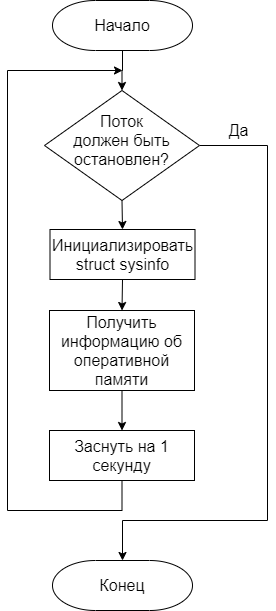
\includegraphics[scale=0.5]{jpg/kthread.png}
	\end{center}
	\captionsetup{justification=centering}
	\caption{Схема алгоритма работы потока}
	\label{fig:kthread}
\end{figure}

Поток ядра находится в состоянии сна и, просыпаясь каждые 10 секунд, фиксирует информацию о свободной и занятой оперативной памяти.

\subsection{Алгоритм перехвата системного вызова}

На рисунках \ref{fig:ftrace_algo_p1}-\ref{fig:ftrace_algo_p2} представлен алгоритм перехвата системных вызовов на примере sys\_clone.

\begin{figure}[h]
	\begin{center}
		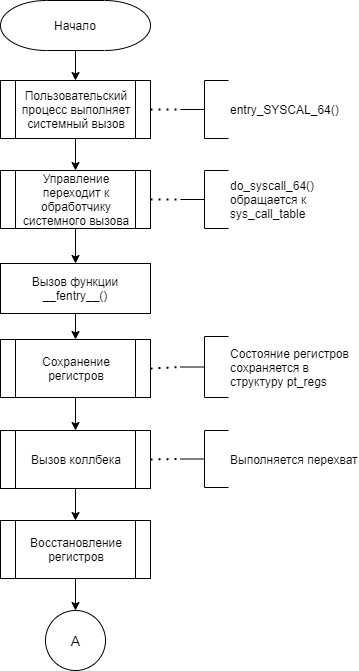
\includegraphics[scale=0.6]{jpg/ftrace_algo-Page-1.jpg}
	\end{center}
	\caption{Алгоритм перехвата системного вызова (ч.~1)}
	\label{fig:ftrace_algo_p1}
\end{figure}

\begin{figure}[h]
	\begin{center}
		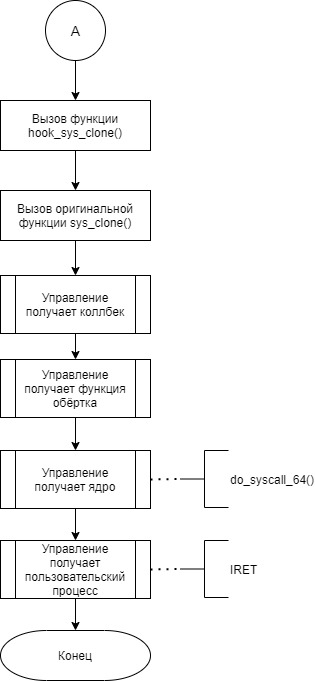
\includegraphics[scale=0.6]{jpg/ftrace_algo-Page-2.jpg}
	\end{center}
	\caption{Алгоритм перехвата системного вызова (ч.~2)}
	\label{fig:ftrace_algo_p2}
\end{figure}

\newpage

\begin{enumerate}
	\item Пользовательский процесс выполняет инструкцию SYSCALL. С помощью этой инструкции выполняется переход в режим ядра и управление передаётся низкоуровневому обработчику системных вызовов\\ entry\_SYSCALL\_64(). Этот обработчик отвечает за все системные вызовы 64-битных программ на 64-битных машинах.
	
	\item Управление переходит к обработчику системного вызова. Ядро передаёт управление функции do\_syscall\_64(). Эта функция обращается к таблице обработчиков системных вызовов sys\_call\_table и с помощью неё вызывает конкретный обработчик системного вызова -- sys\_clone().
	
	\item Вызывается ftrace. В начале каждой функции ядра находится вызов функции \_\_fentry\_\_(), реализованная фреймворком ftrace. Перед этим состояние регистров сохраняется в специальную структуру pt\_regs.
	
	\item ftrace вызывает разработанный коллбек.
	
	\item Коллбек выполняет перехват. Коллбек анализирует значение  parent\_ip и выполняет перехват, обновляя значение регистра rip (указатель на следующую исполняемую инструкцию) в структуре pt\_regs.
	
	\item ftrace восстанавливает значение регистров с помощью структуры pt\_regs. Так как обработчик изменяет значение регистр rip -- это приведёт к передачу управления по новому адресу.
	
	\item Управление получает функция обёртка. Благодаря безусловному переходу, управление получает наша функция hook\_sys\_clone(), а не оригинальная функция sys\_clone(). При этом всё остальное состояние процессора и памяти остаётся без изменений -- функция получает все аргументы оригинального обработчика и при завершении вернёт управление в функцию do\_syscall\_64().
	
	\item Функция обёртка вызывает оригинальную функцию. Функция\\ hook\_sys\_clone() может проанализировать аргументы и контекст системного вызова и запретить или разрешить процессу его выполнение. В случае его запрета, функция просто возвращает код ошибки. Иначе -- вызывает оригинальный обработчик sys\_clone() повторно, с помощью указателя real\_sys\_clone, который был сохранён при настройке перехвата.
	
	\item Управление получает коллбек. Как и при первом вызове sys\_clone(), управление проходит через ftrace и передается в коллбек.
	
	\item Коллбек ничего не делает. В этот раз функция sys\_clone() вызывается разработанной функцией hook\_sys\_clone(), а не ядром из функции\\ do\_syscall\_64(). Коллбек не модифицирует регистры и выполнение функции sys\_clone() продолжается как обычно.
	
	\item Управление передаётся функции обёртке.
	
	\item Управление передаётся ядру. Функция hook\_sys\_clone() завершается и управление переходит к do\_syscall\_64().
	
	\item Управление возвращает в пользовательский процесс. Ядро выполняет инструкцию IRET, устанавливая регистры для нового пользовательского процесса и переводя центральный процессор в режим исполнения пользовательского кода.
\end{enumerate}

\subsection{Алгоритм подсчёта количества системных вызовов}

На рисунке \ref{fig:ftrace_cnt_algo} представлена схема алгоритма подсчёта системных вызовов.

\begin{figure}[h]
	\begin{center}
		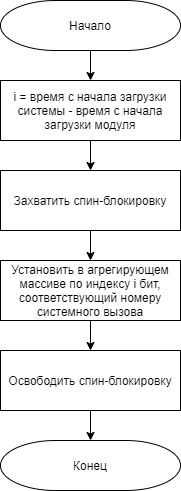
\includegraphics[scale=0.6]{jpg/syscalls_count.jpg}
	\end{center}
	\caption{Алгоритм подсчёта количества системных вызовов}
	\label{fig:ftrace_cnt_algo}
\end{figure}

\newpage

\begin{itemize}
	\item Агрегирующий массив -- это массив на 86400 элементов (что соответствует 24 часам), состоящий из структур, имеющих два поля в виде 64-битных беззнаковых целых чисел. Это позволяет фиксировать до 128 системных вызов в секунду на протяжении 24 часов. Такой массив занимает всего лишь 1350 килобайт оперативной памяти;
	
	\item спин-блокировка необходима с той целью, что несколько системных вызовов могут быть вызваны в один и тот же момент времени -- в таком случае, без блокировки, агрегирующий массив потеряет часть данных.
\end{itemize}

\subsection{Структура ftrace\_ops и функция коллбека}

Для регистрации функции коллбека необходима структура ftrace\_ops~\cite{ftrace_hook}. Структура приведена в листинге~\ref{lst:ftraceops}.

\begin{lstlisting}[label={lst:ftraceops}, caption={структура ftrace\_ops}]
	struct ftrace_ops ops = {
		.func    = callback_func,
		.flags   = FTRACE_FLAGS
		.private = any_private_data_structure,
	};
\end{lstlisting}

Эта структура используется, чтобы сообщить ftrace, какую функцию следует вызывать в качестве коллбека, а также какие меры защиты будут выполняться коллбеком. Поля flags и private являются необязательными.

Включение отслеживания вызовов:

\begin{lstlisting}
	register_ftrace_function(&ops);
\end{lstlisting}

Отключение отслеживания вызовов:

\begin{lstlisting}
	unregister_ftrace_function(&ops);
\end{lstlisting}

Прототип функции коллбека выглядит следующим образом:

\begin{lstlisting}
	void callback_func(unsigned long ip, unsigned long parent_ip, struct ftrace_ops *op, struct pt_regs *regs);
\end{lstlisting}

\begin{itemize}
	\item ip -- указатель инструкции перехватываемой функции;
	
	\item parent\_ip -- указатель инструкции функции, вызвавшей перехватываемую функцию;
	
	\item op -- указатель на ftrace\_ops;
	
	\item regs -- если в структуре ftrace\_ops установлены флаги\\ FTRACE\_OPS\_FL\_SAVE\_REGS или\\ FTRACE\_OPS\_FL\_SAVE\_REGS\_IF\_SUPPORTED, то это будет указывать на структуру pt\_regs, как если бы точка останова была размещена в начале функции, которую перехватывал ftrace. В противном случае он либо содержит мусор, либо NULL.
\end{itemize}

\subsection{Точки входа в загружаемый модуль}

Точками входа разрабатываемого загружаемого модуля ядра будут являться функции инициализации и выхода из модуля.

При инициализации модуля создаются необходимые для сохранения результатов директория и файлы в /proc, создается и запускается поток ядра для подсчета объема свободной и занятой оперативной памяти и устанавливаются хуки для перехвата системных вызовов.

Функция выхода из модуля в свою очередь будет предназначена для остановки потока, удаления созданных директории и файлов в /proc и удаления установленных хуков.

\subsection{Структура ПО}

На рисунке \ref{fig:sw_structure} представлена структура разрабатываемого программного обеспечения.

\begin{figure}[h]
	\begin{center}
		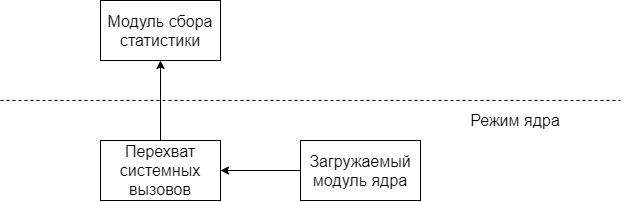
\includegraphics[scale=0.75]{jpg/software_structure.jpg}
	\end{center}
	\caption{Структура программного обеспечения}
	\label{fig:sw_structure}
\end{figure}
\section{Технологическая часть}

\subsection{Выбор языка программирования}

В качестве языка программирования был выбран язык C~\cite{c99}. Данный выбор обусловлен тем, что исходный код ядра Linux, все его модули и драйверы написаны на этом языке.

В качестве компилятора был выбран gcc~\cite{gcc}.

\subsection{Информация о памяти в системе}

Для сбора информации о доступной и свободной памяти в системе запускается отдельный поток ядра, который находится в состоянии сна и,
просыпаясь каждые 10 секунд, фиксирует эту информацию в результирующий массив. В листинге \ref{lst:thread} представлена реализация этого потока, а в листинге \ref{lst:threadinit} его инициализация.

\begin{lstlisting}[label={lst:thread}, caption={реализация функции сохраняющей информацию о памяти}]
	mem_info_t mem_info_array[MEMORY_ARRAY_SIZE];
	int mem_info_calls_cnt;
	
	int memory_cnt_task_handler_fn(void *args) {
		struct sysinfo i;
		struct timespec64 t;
		
		ENTER_LOG();
		
		allow_signal(SIGKILL);
		
		while (!kthread_should_stop()) {
			si_meminfo(&i);
			
			ktime_get_real_ts64(&t);
			
			mem_info_array[mem_info_calls_cnt].free = i.freeram;
			mem_info_array[mem_info_calls_cnt].available = si_mem_available();
			mem_info_array[mem_info_calls_cnt++].time_secs = t.tv_sec;
			
			ssleep(10);
			
			if (signal_pending(worker_task)) {
				break;
			}
		}
		
		EXIT_LOG();
		do_exit(0);
		return 0;
	}
\end{lstlisting}

\begin{lstlisting}[label={lst:threadinit}, caption={инициализация потока ядра}]
	cpu = get_cpu();
	worker_task = kthread_create(memory_cnt_task_handler_fn, NULL, "memory counter thread");
	kthread_bind(worker_task, cpu);
	
	if (worker_task == NULL) {
		cleanup();
		return -1;
	}
	
	wake_up_process(worker_task);
	return 0;
\end{lstlisting}

\subsection{Поиск адреса перехватываемой функции}

Для корректной работы ftrace необходимо найти и сохранить адрес функции, которую будет перехватывать разрабатываемый модуль ядра. 

В старых версиях ядра (в версии ядра 5.7.0 данная функция перестала быть экспортируемой \cite{kallsyms-removed}) найти адрес функции можно было с помощью функции kallsyms\_lookup\_name() -- списка всех символов в ядре, в том числе не экспортируемых для модулей. Так как модуль ядра разрабатывался на системе с версией ядра 5.15.0, воспользоваться данным способом было нельзя. Поэтому использовался интерфейс kprobes.

Из-за того, что данный способ имеет больше накладных расходов, чем поиск с помощью kallsyms\_lookup\_name() (требуется регистрация и удаление kprobes в системе), для версий ядра ниже 5.7.0 поиск адреса производится с помощью kallsyms\_lookup\_name(). 

Реализация функции lookup\_name(), возвращающей адрес перехватываемой функции по её названию, представлена в листинге \ref{lst:lookup_name}.

\begin{lstlisting}[label=lst:lookup_name, caption=Реализация функции lookup\_name()]
	#if LINUX_VERSION_CODE >= KERNEL_VERSION(5,7,0)
	static unsigned long lookup_name(const char *name)
	{
		struct kprobe kp = {
			.symbol_name = name
		};
		unsigned long retval;
		
		ENTER_LOG();
		
		if (register_kprobe(&kp) < 0) {
			EXIT_LOG();
			return 0;
		}
		
		retval = (unsigned long) kp.addr;
		unregister_kprobe(&kp);
		
		EXIT_LOG();
		
		return retval;
	}
	#else
	static unsigned long lookup_name(const char *name)
	{
		unsigned long retval;
		
		ENTER_LOG();
		retval = kallsyms_lookup_name(name);
		EXIT_LOG();
		
		return retval;
	}
	#endif
\end{lstlisting}

\subsection{Инициализация ftrace}

В листинге \ref{lst:install_hook} представлена реализация функции, которая инициализирует структуру ftrace\_ops.

\begin{lstlisting}[label=lst:install_hook, caption=Реализация функции install\_hook()]
	static int install_hook(struct ftrace_hook *hook) {
		int rc;
		
		ENTER_LOG();
		
		if ((rc = resolve_hook_address(hook))) {
			EXIT_LOG();
			return rc;
		}
		
		hook->ops.func = ftrace_thunk; 
		hook->ops.flags = FTRACE_OPS_FL_SAVE_REGS
		| FTRACE_OPS_FL_RECURSION
		| FTRACE_OPS_FL_IPMODIFY;
		
		if ((rc = ftrace_set_filter_ip(&hook->ops, hook->address, 0, 0))) {
			pr_debug("ftrace_set_filter_ip() failed: %d\n", rc);
			return rc;
		}
		
		if ((rc = register_ftrace_function(&hook->ops))) {
			pr_debug("register_ftrace_function() failed: %d\n", rc);
			ftrace_set_filter_ip(&hook->ops, hook->address, 1, 0);
		}
		
		EXIT_LOG();
		
		return rc;
	}
\end{lstlisting}

В листинге \ref{lst:remove_hook} представлена реализация отключения перехвата функции.

\begin{lstlisting}[label=lst:remove_hook, caption=Реализация функции remove\_hook()]
	static void remove_hook(struct ftrace_hook *hook) {
		int rc;
		
		ENTER_LOG();
		
		if (hook->address == 0x00) {
			EXIT_LOG();
			return;
		}
		
		if ((rc = unregister_ftrace_function(&hook->ops))) {
			pr_debug("unregister_ftrace_function() failed: %d\n", rc);
		}
		
		if ((rc = ftrace_set_filter_ip(&hook->ops, hook->address, 1, 0))) {
			pr_debug("ftrace_set_filter_ip() failed: %d\n", rc);
		}
		
		hook->address = 0x00;
		
		EXIT_LOG();
	}
\end{lstlisting}

\subsection{Функции обёртки}

При объявлении функций обёрток, которые будут запущены вместо перехватываемой функции, необходимо в точности соблюдать сигнатуру. Оригинальные описания функций были взяты из исходных кодов ядра Linux. 

В листинге \ref{lst:sys_execve} представлена реализация функции обёртки на примере sys\_clone().

\begin{lstlisting}[label=lst:sys_execve, caption=Реализация функции обёртки]
	static asmlinkage long (*real_sys_clone)(unsigned long clone_flags,
	unsigned long newsp, int __user *parent_tidptr,
	int __user *child_tidptr, unsigned long tls);
	
	static asmlinkage long hook_sys_clone(unsigned long clone_flags,
	unsigned long newsp, int __user *parent_tidptr,
	int __user *child_tidptr, unsigned long tls)
	{
		update_syscall_array(SYS_CLONE_NUM);
		return real_sys_clone(clone_flags, newsp, parent_tidptr, child_tidptr, tls);
	}
\end{lstlisting}

В листинге \ref{lst:update_syscall_array} представлена реализация функции которая обновляет массив, хранящий количество системных вызовов за последние 24 часа.

\begin{lstlisting}[label=lst:update_syscall_array, caption=Реализация функции update\_syscall\_array()]
	static DEFINE_SPINLOCK(my_lock);
	
	static void inline update_syscall_array(int syscall_num) {
		ktime_t time;
		
		time = ktime_get_boottime_seconds() - start_time;
		
		spin_lock(&my_lock);
		
		if (syscall_num < 64) {
			syscalls_time_array[time % TIME_ARRAY_SIZE].p1 |= 1UL << syscall_num;
		} else {
			syscalls_time_array[time % TIME_ARRAY_SIZE].p2 |= 1UL << (syscall_num % 64);
		}
		
		spin_unlock(&my_lock);
	}
\end{lstlisting}

\subsection{Получение информации о количестве системных вызовов}

В листинге \ref{lst:syscall_proc} представлена реализация функций, которые агрегируют информацию о системных вызовах (данные массива update\_syscall\_array) и предоставляют ее в читаемом для пользователя виде.

\begin{lstlisting}[label=lst:syscall_proc, caption=Реализация функций агрегации данных о системных вызовах, language=c]
	static inline void walk_bits_and_find_syscalls(struct seq_file *m, uint64_t num, int syscalls_arr_cnt[]) {
		int i;
		
		for (i = 0; i < 64; i++) {
			if (num & (1UL << i)) {
				syscalls_arr_cnt[i]++;
			}
		}
	}
	
	void print_syscall_statistics(struct seq_file *m, const ktime_t mstart, ktime_t range) {
		int syscalls_arr_cnt[128];
		uint64_t tmp;
		size_t i;
		ktime_t uptime;
		
		memset((void*)syscalls_arr_cnt, 0, 128 * sizeof(int));
		uptime = ktime_get_boottime_seconds() - mstart;
		
		if (uptime < range) {
			range = uptime;
		}
		
		for (i = 0; i < range; i++) {
			if ((tmp = syscalls_time_array[uptime - i].p1) != 0) {
				walk_bits_and_find_syscalls(m, tmp, syscalls_arr_cnt);
			}
			
			if ((tmp = syscalls_time_array[uptime - i].p2) != 0) {
				walk_bits_and_find_syscalls(m, tmp, syscalls_arr_cnt + 64);
			}
		}
		
		show_int_message(m, "Syscall statistics for the last %d seconds.\n\n", range);
		
		for (i = 0; i < 128; i++) {
			if (syscalls_arr_cnt[i] != 0) {
				show_str_message(m, "%s called ", syscalls_names[i]);
				show_int_message(m, "%d times.\n", syscalls_arr_cnt[i]);
			}
		}
	}
\end{lstlisting}

\subsection{Детали реализации}

В листингах \ref{lst:mdinit}-\ref{lst:cleanup} представлена реализация точек входа в загружаемый модуль.

\begin{lstlisting}[label={lst:mdinit}, caption={функция инициализации модуля}]
	static int __init md_init(void) {
		int rc;
		int cpu;
		
		ENTER_LOG();
		
		if ((rc = proc_init())) {
			return rc;
		}
		
		if ((rc = install_hooks())) {
			cleanup();
			return rc;
		}
		
		start_time = ktime_get_boottime_seconds();
		
		cpu = get_cpu();
		worker_task = kthread_create(memory_cnt_task_handler_fn, NULL, "memory counter thread");
		kthread_bind(worker_task, cpu);
		
		if (worker_task == NULL) {
			cleanup();
			return -1;
		}
		
		wake_up_process(worker_task);
		
		printk("%s: module loaded\n", MODULE_NAME);
		EXIT_LOG();
		
		return 0;
	}
\end{lstlisting}

\begin{lstlisting}[label={lst:mdexit}, caption={функция выхода из модуля}]
	static void __exit md_exit(void) { 
		cleanup();
		
		printk("%s: module unloaded\n", MODULE_NAME); 
	}
\end{lstlisting}

\begin{lstlisting}[label={lst:cleanup}, caption={функция cleanup()}]
	static void cleanup(void) {
		ENTER_LOG();
		
		if (worker_task) {
			kthread_stop(worker_task);
		}
		
		if (proc_mem_file != NULL) {
			remove_proc_entry("memory", proc_root);
		}
		
		if (proc_syscall_file != NULL) {
			remove_proc_entry("syscalls", proc_root);
		}
		
		if (proc_root != NULL) {
			remove_proc_entry(MODULE_NAME, NULL);
		}
		
		remove_hooks();
		
		EXIT_LOG();
	}
\end{lstlisting}

Make файл для компиляции и сборки разработанного загружаемого модуля ядра представлен в листинге \ref{lst:makefile}.

\begin{lstlisting}[label={lst:makefile}, caption={реализация make файла}]
	KPATH := /lib/modules/$(shell uname -r)/build
	MDIR := $(shell pwd)
	
	obj-m += monitor.o
	monitor-y := monitor_main.o stat.o hooks.o log.o
	EXTRA_CFLAGS=-I$(PWD)/inc
	
	all:
	make -C $(KPATH) M=$(MDIR) modules
	
	clean:
	make -C $(KPATH) M=$(MDIR) clean
	
	load:
	sudo insmod monitor.ko
	
	unload:
	sudo rmmod monitor.ko
	
	info:
	modinfo monitor.ko
	
	logs:
	sudo dmesg | tail -n60 | grep monitor:
\end{lstlisting}

\section{Исследовательская часть}

\subsection{Результаты работы разработанного ПО}

На рисунках \ref{fig:example_mem}-\ref{fig:example_syscalls} представлены примеры работы модуля, а на рисунке \ref{fig:free-m} -- сравнение результатов получения информации об объеме оперативной памяти с результатами команды <<free -m>> (у последней все объемы указаны в Мб).

\begin{figure}[h!]
	\begin{center}
		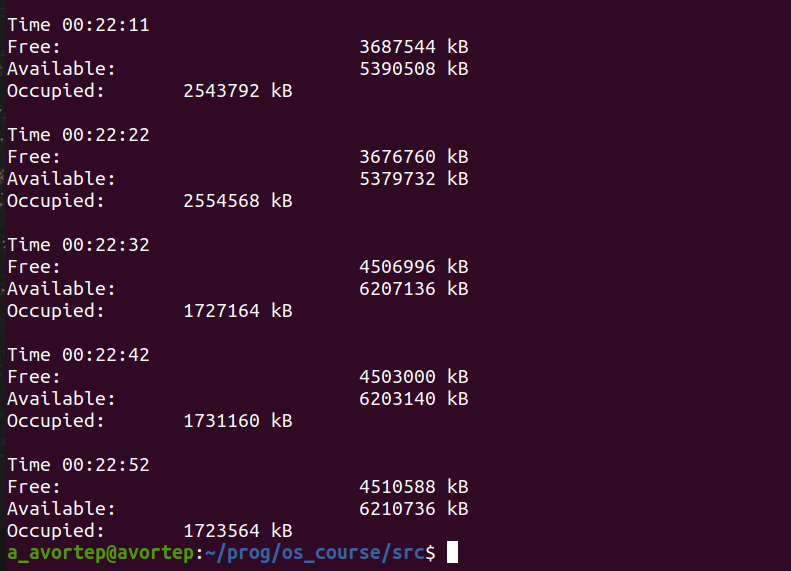
\includegraphics[scale=0.4]{jpg/2.png}
	\end{center}
	\captionsetup{justification=centering}
	\caption{Информация об оперативной памяти в системе}
	\label{fig:example_mem}
\end{figure}

\begin{figure}[h!]
	\begin{center}
		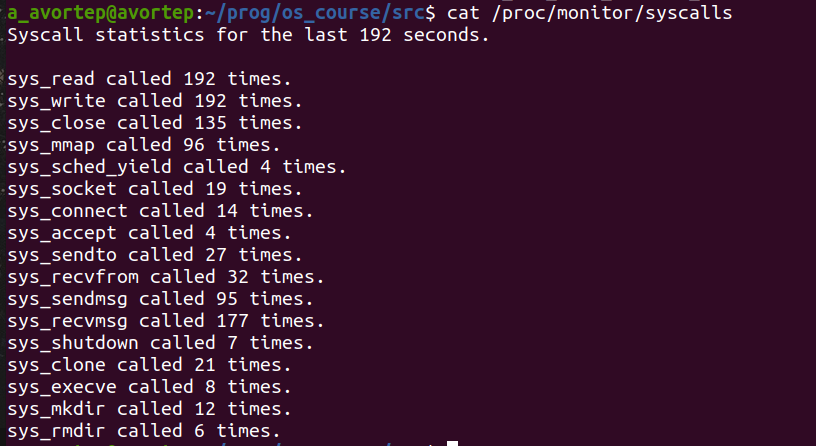
\includegraphics[scale=0.4]{jpg/cat_syscalls.png}
	\end{center}
	\captionsetup{justification=centering}
	\caption{Информация о количестве системных вызовов за последние 192 секунды}
	\label{fig:example_syscalls}
\end{figure}

\begin{figure}[h!]
	\begin{center}
		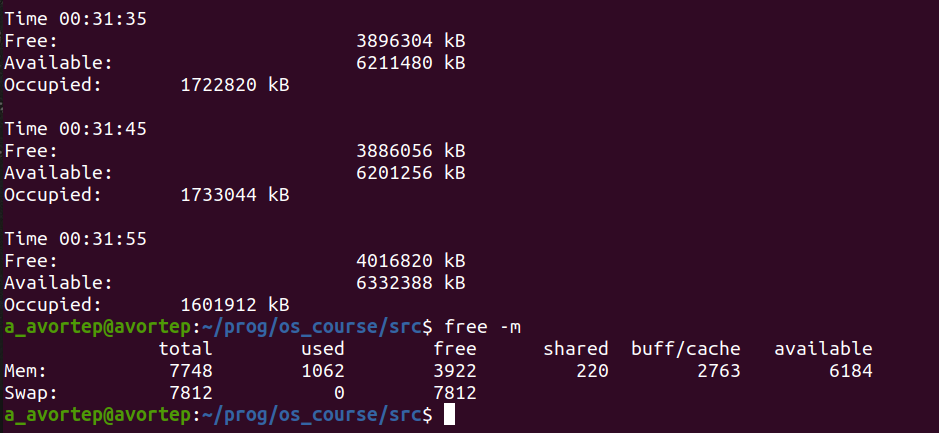
\includegraphics[scale=0.45]{jpg/3.png}
	\end{center}
	\captionsetup{justification=centering}
	\caption{Результаты работы команды <<free -m>>}
	\label{fig:free-m}
\end{figure}

На рисунке \ref{fig:graphic} представлена визуализация данных о свободной, доступной и занятой памяти в системе, полученных из разработанного модуля ядра.

\begin{figure}[h!]
	\begin{center}
		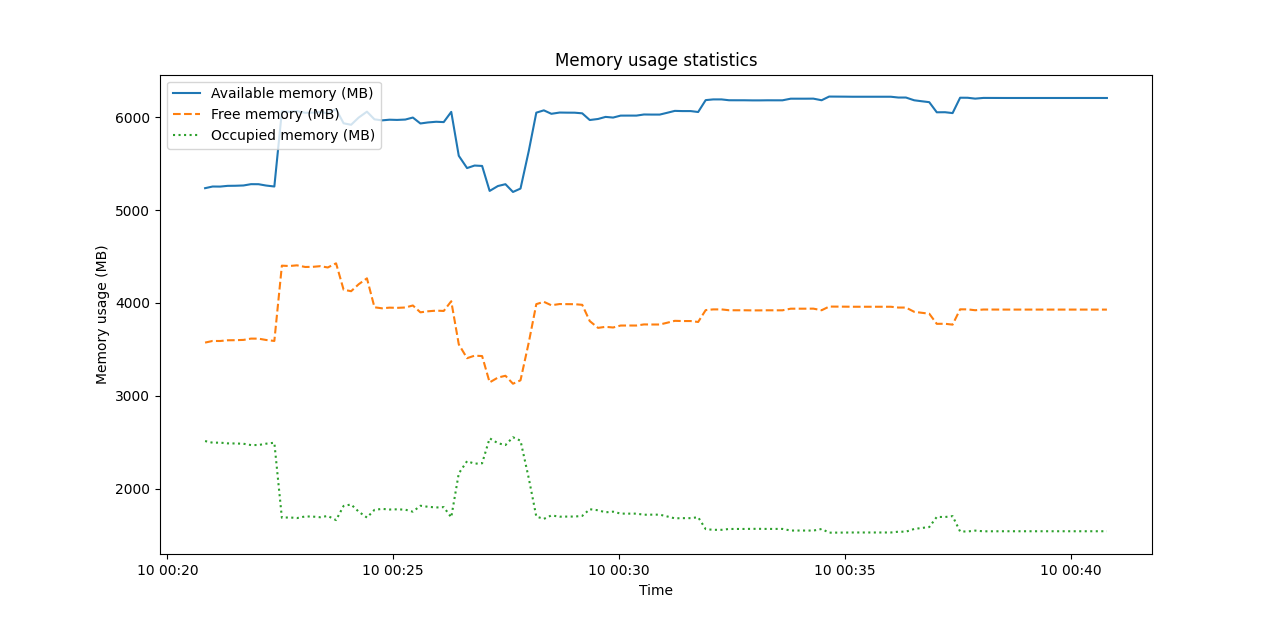
\includegraphics[scale=0.55]{jpg/memory_usage.png}
	\end{center}
	\captionsetup{justification=centering}
	\caption{Визуализация данных о памяти за 20 минут}
	\label{fig:graphic}
\end{figure}

\newpage

\subsection{Анализ результатов}

На основе рисунка \ref{fig:free-m} можно сделать вывод, что результаты работы разработанного загружаемого модуля ядра совпадают с результатами работы команды <<free -m>>. Следовательно, результаты корректны.

По рисунку \ref{fig:graphic} видно, как изменялась загруженность памяти в течение 20 минут. В моменты резкого спада количества занятой оперативной памяти было закрыто несколько приложений, а в моменты роста -- наоборот, открыто.


\specsection{Заключение}

Цель курсового проекта достигнута. В ходе проделанной работы был разработан загружаемый модуль ядра, предоставляющий информацию о загруженности оперативной памяти системы.

Для этого были изучены структуры и функции ядра, которые предоставляют информацию о памяти. На основе чего был разработан, а затем реализован алгоритм работы программы.

Помимо этого были также приведены и проанализированы результаты работы ПО.

% говно литература для тест ВКР
\specsection{СПИСОК ИСПОЛЬЗОВАННЫХ ИСТОЧНИКОВ}

\begingroup
\renewcommand{\section}[2]{}
\begin{thebibliography}{}

\bibitem{linux}
Linux -- Operating System [Электронный ресурс]. -- Режим доступа: \url {https://www.linux.org/} (дата обращения: 20.12.2022).

\bibitem{commands}
Использование оперативной памяти в Linux [Электронный ресурс]. -- Режим доступа: \url {https://losst.pro/ispolzovanie-operativnoj-pamyati-linux} (дата обращения: 20.12.2022).

\bibitem{gnome}
System Monitor – Apps for GNOME [Электронный ресурс]. -- Режим доступа: \url {https://apps.gnome.org/ru/app/gnome-system-monitor/} (дата обращения: 23.12.2022).

\bibitem{meminfo}
The /proc/meminfo File in Linux [Электронный ресурс]. -- Режим доступа: \url {https://www.baeldung.com/linux/proc-meminfo} (дата обращения: 24.12.2022).

\bibitem{sysinfo}

include/uapi/linux/sysinfo.h - Linux source code (v5.15) [Электронный ресурс]. -- Режим доступа: \url {https://elixir.bootlin.com/linux/v5.15/source/include/uapi/linux/sysinfo.h} (дата обращения: 24.12.2022).

\bibitem{habr-profiling-linux}

Механизмы профилирования Linux [Электронный ресурс]. -- Режим доступа: \url {https://habr.com/ru/company/metrotek/blog/261003/} (дата обращения: 13.02.2023).

\bibitem{kprobes}

Kernel Probes (Kprobes) [Электронный ресурс]. -- Режим доступа: \url {https://www.kernel.org/doc/html/latest/trace/kprobes.html} (дата обращения: 14.02.2023).

\bibitem{kernel-tracepoints}

Using the Linux Kernel Tracepoints [Электронный ресурс]. -- Режим доступа: \url {https://www.kernel.org/doc/html/latest/trace/tracepoints.html} (дата обращения: 14.02.2023).

\bibitem{ftrace}

Using ftrace | Android Open Source Project [Электронный ресурс]. -- Режим доступа: \url {https://source.android.com/devices/tech/debug/ftrace} (дата обращения: 14.02.2023).

\bibitem{ftrace-habr}

Трассировка ядра с ftrace [Электронный ресурс]. -- Режим доступа: \url {https://habr.com/ru/company/selectel/blog/280322/} (дата обращения: 14.02.2023).

\bibitem{ftrace_hook}

Using ftrace to hook to functions [Электронный ресурс]. -- Режим доступа: \url {https://www.kernel.org/doc/html/latest/trace/ftrace-uses.html} (дата обращения: 15.02.2023).

\bibitem{c99}

C99 standard note [Электронный ресурс]. -- Режим доступа: \url {https://www.open-std.org/jtc1/sc22/wg14/www/docs/n1256.pdf} (дата обращения: 17.01.2023).

\bibitem{gcc}

GCC, the GNU Compiler Collection [Электронный ресурс]. -- Режим доступа: \url {https://gcc.gnu.org/} (дата обращения: 17.01.2023).

\bibitem{kallsyms-removed}

Unexporting kallsyms\_lookup\_name() [Электронный ресурс]. -- Режим доступа: \url {https://lwn.net/Articles/813350/} (дата обращения: 15.02.2023).

\end{thebibliography}
\endgroup

% норм по феншую
%\bibliographystyle{utf8gost705u}
%\renewcommand{\refname}{СПИСОК ИСПОЛЬЗОВАННЫХ ИСТОЧНИКОВ}
%\bibliography{bibliography}

\anonsection{ПРИЛОЖЕНИЕ А}

\begin{lstlisting}[caption={листинг файла monitor\_main.c}]
	#include <linux/module.h>
	#include <linux/proc_fs.h> 
	#include <linux/time.h>
	#include <linux/kthread.h>
	
	#include "hooks.h"
	#include "memory.h"
	#include "stat.h"
	
	MODULE_LICENSE("GPL");
	MODULE_AUTHOR("Petrova Anna");
	MODULE_DESCRIPTION("A utility for monitoring RAM usage and number of syscalls");
	
	static struct proc_dir_entry *proc_root = NULL;
	static struct proc_dir_entry *proc_mem_file = NULL, *proc_syscall_file = NULL;
	static struct task_struct *worker_task = NULL;
	
	extern ktime_t start_time;
	/* default syscall range value is 10 min */
	static ktime_t syscalls_range_in_seconds = 600;
	
	static int show_memory(struct seq_file *m, void *v) {
		print_memory_statistics(m);
		return 0;
	}
	
	static int proc_memory_open(struct inode *sp_inode, struct file *sp_file) {
		return single_open(sp_file, show_memory, NULL);
	}
	
	static int show_syscalls(struct seq_file *m, void *v) {
		print_syscall_statistics(m, start_time, syscalls_range_in_seconds);
		return 0;
	}
	
	static int proc_syscalls_open(struct inode *sp_inode, struct file *sp_file) {
		return single_open(sp_file, show_syscalls, NULL);
	}
	
	static int proc_release(struct inode *sp_node, struct file *sp_file) {
		return 0;
	}
	
	mem_info_t mem_info_array[MEMORY_ARRAY_SIZE];
	int mem_info_calls_cnt;
	
	int memory_cnt_task_handler_fn(void *args) {
		struct sysinfo i;
		struct timespec64 t;
		
		ENTER_LOG();
		
		allow_signal(SIGKILL);
		
		while (!kthread_should_stop()) {
			si_meminfo(&i);
			
			ktime_get_real_ts64(&t);
			
			mem_info_array[mem_info_calls_cnt].free = i.freeram;
			mem_info_array[mem_info_calls_cnt].available = si_mem_available();
			mem_info_array[mem_info_calls_cnt++].time_secs = t.tv_sec;
			
			ssleep(10);
			
			if (signal_pending(worker_task)) {
				break;
			}
		}
		
		EXIT_LOG();
		do_exit(0);
		return 0;
	}
	
	#define CHAR_TO_INT(ch) (ch - '0')
	
	static ktime_t convert_strf_to_seconds(char buf[]) {
		/* time format: xxhyymzzs. For example: 01h23m45s */
		ktime_t hours, min, secs;
		
		hours = CHAR_TO_INT(buf[0]) * 10 + CHAR_TO_INT(buf[1]);
		min = CHAR_TO_INT(buf[3]) * 10 + CHAR_TO_INT(buf[4]);
		secs = CHAR_TO_INT(buf[6]) * 10 + CHAR_TO_INT(buf[7]);
		
		return hours * 60 * 60 + min * 60 + secs;
	}
	
	static ssize_t proc_syscall_write(struct file *file, const char __user *buf, size_t len, loff_t *ppos) {
		char syscalls_time_range[10];
		
		ENTER_LOG();
		
		if (copy_from_user(&syscalls_time_range, buf, len) != 0) {
			EXIT_LOG()
			return -EFAULT;
		}
		
		syscalls_range_in_seconds = convert_strf_to_seconds(syscalls_time_range);
		
		EXIT_LOG();
		return len;
	}
	
	static const struct proc_ops mem_ops = {
		proc_read: seq_read,
		proc_open: proc_memory_open,
		proc_release: proc_release,
	};
	
	static const struct proc_ops syscalls_ops = {
		proc_read: seq_read,
		proc_open: proc_syscalls_open,
		proc_release: proc_release,
		proc_write: proc_syscall_write,
	};
	
	static void cleanup(void) {
		ENTER_LOG();
		
		if (worker_task) {
			kthread_stop(worker_task);
		}
		
		if (proc_mem_file != NULL) {
			remove_proc_entry("memory", proc_root);
		}
		
		if (proc_syscall_file != NULL) {
			remove_proc_entry("syscalls", proc_root);
		}
		
		if (proc_root != NULL) {
			remove_proc_entry(MODULE_NAME, NULL);
		}
		
		remove_hooks();
		
		EXIT_LOG();
	}
	
	static int proc_init(void) {
		ENTER_LOG();
		
		if ((proc_root = proc_mkdir(MODULE_NAME, NULL)) == NULL) {
			goto err;
		}
		
		if ((proc_mem_file = proc_create("memory", 066, proc_root, &mem_ops)) == NULL) {
			goto err;
		}
		
		if ((proc_syscall_file = proc_create("syscalls", 066, proc_root, &syscalls_ops)) == NULL)
		{
			goto err;
		}
		
		EXIT_LOG();
		return 0;
		
		err:
		cleanup();
		EXIT_LOG();
		return -ENOMEM;
	}
	
	static int __init md_init(void) {
		int rc;
		int cpu;
		
		ENTER_LOG();
		
		if ((rc = proc_init())) {
			return rc;
		}
		
		if ((rc = install_hooks())) {
			cleanup();
			return rc;
		}
		
		start_time = ktime_get_boottime_seconds();
		
		cpu = get_cpu();
		worker_task = kthread_create(memory_cnt_task_handler_fn, NULL, "memory counter thread");
		kthread_bind(worker_task, cpu);
		
		if (worker_task == NULL) {
			cleanup();
			return -1;
		}
		
		wake_up_process(worker_task);
		
		printk("%s: module loaded\n", MODULE_NAME);
		EXIT_LOG();
		
		return 0;
	}
	
	static void __exit md_exit(void) { 
		cleanup();
		
		printk("%s: module unloaded\n", MODULE_NAME); 
	}
	
	module_init(md_init);
	module_exit(md_exit);
\end{lstlisting}

\begin{lstlisting}[caption={листинг файла stat.c}]
	#include "stat.h"
	
	static inline long convert_to_kb(const long n) {
		return n << (PAGE_SHIFT - 10);
	}
	
	void print_memory_statistics(struct seq_file *m) {
		struct sysinfo info;
		long long secs;
		long sys_occupied;
		int i;
		
		ENTER_LOG();
		
		si_meminfo(&info);
		show_int_message(m, "Memory total: \t%ld kB\n", convert_to_kb(info.totalram));
		
		for (i = 0; i < mem_info_calls_cnt; i++) {
			secs = mem_info_array[i].time_secs;
			show_int3_message(m, "\nTime %.2llu:%.2llu:%.2llu\n", (secs / 3600 + 3) % 24, secs / 60 % 60, secs % 60);
			show_int_message(m, "Free:      \t\t\t%ld kB\n", convert_to_kb(mem_info_array[i].free));
			show_int_message(m, "Available: \t\t\t%ld kB\n", convert_to_kb(mem_info_array[i].available));
			sys_occupied = convert_to_kb(info.totalram) - convert_to_kb(mem_info_array[i].available);
			show_int_message(m, "Occupied: \t%ld kB\n", sys_occupied);
		}
		
		EXIT_LOG();
	}
	
	syscalls_info_t syscalls_time_array[TIME_ARRAY_SIZE];
	
	static const char *syscalls_names[] = {
		"sys_read", // 0 
		"sys_write", 
		"sys_open",
		"sys_close",
		"sys_newstat", // 4 
		"sys_newfstat",
		"sys_newlstat",
		"sys_poll",
		"sys_lseek",
		"sys_mmap", // 9 
		"sys_mprotect",
		"sys_munmap",
		"sys_brk",
		"sys_rt_sigaction",
		"sys_rt_sigprocmask", // 14 
		"stub_rt_sigreturn",
		"sys_ioctl",
		"sys_pread64",
		"sys_pwrite64",
		"sys_readv", // 19 
		"sys_writev",
		"sys_access",
		"sys_pipe",
		"sys_select",
		"sys_sched_yield", // 24 
		"sys_mremap",
		"sys_msync",
		"sys_mincore",
		"sys_madvise",
		"sys_shmget", // 29 
		"sys_shmat",
		"sys_shmctl",
		"sys_dup",
		"sys_dup2",
		"sys_pause", // 34 
		"sys_nanosleep",
		"sys_gettimer",
		"sys_alarm",
		"sys_settimer",
		"sys_getpid", // 39 
		"sys_sendfile64",
		"sys_socket",
		"sys_connect",
		"sys_accept",
		"sys_sendto", // 44 
		"sys_recvfrom",
		"sys_sendmsg",
		"sys_recvmsg",
		"sys_shutdown",
		"sys_bind", // 49
		"sys_listen",
		"sys_getsockname",
		"sys_getpeername",
		"sys_socketpair",
		"sys_setsockopt", // 54 
		"sys_getsockopt",
		"sys_clone",
		"sys_fork",
		"sys_vfork",
		"sys_execve", // 59 
		"sys_exit",
		"sys_wait4",
		"sys_kill",
		"sys_newuname",
		"sys_semget", // 64 
		"sys_semop",
		"sys_semctl",
		"sys_shmdt",
		"sys_msgget",
		"sys_msgsnd", // 69 
		"sys_msgrcv",
		"sys_msgctl",
		"sys_fcntl",
		"sys_flock",
		"sys_fsync", // 74 
		"sys_fdatasync",
		"sys_truncate",
		"sys_ftruncate",
		"sys_getdents",
		"sys_getcwd", // 79 
		"sys_chdir",
		"sys_fchdir",
		"sys_rename",
		"sys_mkdir",
		"sys_rmdir", // 84 
		"sys_creat",
		"sys_link",
		"sys_unlink",
		"sys_symlink",
		"sys_readlink", // 89 
		"sys_chmod",
		"sys_fchmod",
		"sys_chown",
		"sys_fchown",
		"sys_lchown", // 94 
		"sys_umask",
		"sysgettimeofday",
		"sys_getrlimit",
		"sys_getrusage",
		"sys_sysinfo", // 99 
		"sys_times",
		"sys_ptrace",
		"sys_getuid",
		"sys_syslog",
		"sys_getgid", // 104 
		"sys_setuid",
		"sys_setgid",
		"sys_geteuid",
		"sys_getegid",
		"sys_getpgid", // 109 
		"sys_getppid",
		"sys_getpgrp",
		"sys_setsid",
		"sys_setreuid",
		"sys_setregid", // 114 
		"sys_getgroups",
		"sys_setgroups",
		"sys_setresuid",
		"sys_getresuid",
		"sys_setresgid", // 119 
		"sys_getresgid",
		"sys_getpgid",
		"sys_setfsuid",
		"sys_setfsgid",
		"sys_getsid", // 124 
		"sys_capget",  
		"sys_capset",
		"sys_rt_sigpending", // 127 
	};
	
	static inline void walk_bits_and_find_syscalls(struct seq_file *m, uint64_t num, int syscalls_arr_cnt[]) {
		int i;
		
		for (i = 0; i < 64; i++) {
			if (num & (1UL << i)) {
				syscalls_arr_cnt[i]++;
			}
		}
	}
	
	void print_syscall_statistics(struct seq_file *m, const ktime_t mstart, ktime_t range) {
		int syscalls_arr_cnt[128];
		uint64_t tmp;
		size_t i;
		ktime_t uptime;
		
		memset((void*)syscalls_arr_cnt, 0, 128 * sizeof(int));
		uptime = ktime_get_boottime_seconds() - mstart;
		
		if (uptime < range) {
			range = uptime;
		}
		
		for (i = 0; i < range; i++) {
			if ((tmp = syscalls_time_array[uptime - i].p1) != 0) {
				walk_bits_and_find_syscalls(m, tmp, syscalls_arr_cnt);
			}
			
			if ((tmp = syscalls_time_array[uptime - i].p2) != 0) {
				walk_bits_and_find_syscalls(m, tmp, syscalls_arr_cnt + 64);
			}
		}
		
		show_int_message(m, "Syscall statistics for the last %d seconds.\n\n", range);
		
		for (i = 0; i < 128; i++) {
			if (syscalls_arr_cnt[i] != 0) {
				show_str_message(m, "%s called ", syscalls_names[i]);
				show_int_message(m, "%d times.\n", syscalls_arr_cnt[i]);
			}
		}
	}
\end{lstlisting}

\begin{lstlisting}[caption={листинг файла log.c}]
	#include "log.h"
	
	void show_int_message(struct seq_file *m, const char *const f, const long num) {
		char tmp[256];
		int len;
		
		len = snprintf(tmp, 256, f, num);
		seq_write(m, tmp, len);
	}
	
	void show_int3_message(struct seq_file *m, const char *const f, const long n1, const long n2, const long n3) {
		char tmp[256];
		int len;
		
		len = snprintf(tmp, 256, f, n1, n2, n3);
		seq_write(m, tmp, len);
	}
	
	void show_str_message(struct seq_file *m, const char *const f, const char *const s) {
		char tmp[256];
		int len;
		
		len = snprintf(tmp, 256, f, s);
		seq_write(m, tmp, len);
	}
\end{lstlisting}

\begin{lstlisting}[caption={листинг файла memory.h}]
	#ifndef __MEMORY_H__
	#define __MEMORY_H__
	
	#include <linux/kthread.h>
	#include <linux/delay.h>
	#include <linux/time.h>
	
	#include "log.h"
	
	typedef struct mem_struct {
		long available;
		long free;
		long time_secs;
	} mem_info_t;
	
	#define MEMORY_ARRAY_SIZE 8640
	extern mem_info_t mem_info_array[MEMORY_ARRAY_SIZE];
	
	extern int mem_info_calls_cnt;
	
	#endif
\end{lstlisting}

\begin{lstlisting}[caption={листинг файла hooks.c}]
	#include "hooks.h"
	
	#pragma GCC optimize("-fno-optimize-sibling-calls")
	
	#if defined(CONFIG_X86_64) && (LINUX_VERSION_CODE >= KERNEL_VERSION(4,17,0))
	#define PTREGS_SYSCALL_STUBS 1
	#endif
	
	#if LINUX_VERSION_CODE < KERNEL_VERSION(5,11,0)
	#define FTRACE_OPS_FL_RECURSION FTRACE_OPS_FL_RECURSION_SAFE
	#endif
	
	#if LINUX_VERSION_CODE < KERNEL_VERSION(5,11,0)
	#define ftrace_regs pt_regs
	
	static __always_inline struct pt_regs *ftrace_get_regs(struct ftrace_regs *fregs)
	{
		return fregs;
	}
	#endif
	
	ktime_t start_time;
	static DEFINE_SPINLOCK(my_lock);
	
	static void inline update_syscall_array(int syscall_num) {
		ktime_t time;
		
		time = ktime_get_boottime_seconds() - start_time;
		
		spin_lock(&my_lock);
		
		if (syscall_num < 64) {
			syscalls_time_array[time % TIME_ARRAY_SIZE].p1 |= 1UL << syscall_num;
		} else {
			syscalls_time_array[time % TIME_ARRAY_SIZE].p2 |= 1UL << (syscall_num % 64);
		}
		
		spin_unlock(&my_lock);
	}
	
	/* 0 - sys_read */
	#ifdef PTREGS_SYSCALL_STUBS
	static asmlinkage long (*real_sys_read)(struct pt_regs *regs);
	
	static asmlinkage long hook_sys_read(struct pt_regs *regs)
	{
		update_syscall_array(SYS_READ_NUM);
		return real_sys_read(regs);
	}
	#else
	static asmlinkage long (*real_sys_read)(unsigned int fd, char __user *buf, size_t count);
	
	static asmlinkage long hook_sys_read(unsigned int fd, char __user *buf, size_t count)
	{
		update_syscall_array(SYS_READ_NUM);
		return real_sys_read(fd, buf, count);
	}
	#endif
	
	/* 1 - sys_write */
	#ifdef PTREGS_SYSCALL_STUBS
	static asmlinkage long (*real_sys_write)(struct pt_regs *regs);
	
	static asmlinkage long hook_sys_write(struct pt_regs *regs)
	{
		update_syscall_array(SYS_WRITE_NUM);
		return real_sys_write(regs);
	}
	#else
	static asmlinkage long (*real_sys_write)(unsigned int fd, const char __user *buf, size_t count);
	
	static asmlinkage long hook_sys_write(unsigned int fd, const char __user *buf, size_t count)
	{
		update_syscall_array(SYS_WRITE_NUM);
		return real_sys_write(fd, buf, count);
	}
	#endif
	
	/* 2 - sys_open */
	#ifdef PTREGS_SYSCALL_STUBS
	static asmlinkage long (*real_sys_open)(struct pt_regs *regs);
	
	static asmlinkage long hook_sys_open(struct pt_regs *regs)
	{
		update_syscall_array(SYS_OPEN_NUM);
		return real_sys_open(regs);
	}
	#else
	static asmlinkage long (*real_sys_open)(const char __user *filename, int flags, umode_t mode);
	
	static asmlinkage long hook_sys_open(const char __user *filename, int flags, umode_t mode);
	{
		update_syscall_array(SYS_OPEN_NUM);
		return real_sys_open(filename, flags, mode);
	}
	#endif
	
	/* 3 - sys_close */
	#ifdef PTREGS_SYSCALL_STUBS
	static asmlinkage long (*real_sys_close)(struct pt_regs *regs);
	
	static asmlinkage long hook_sys_close(struct pt_regs *regs)
	{
		update_syscall_array(SYS_CLOSE_NUM);
		return real_sys_close(regs);
	}
	#else
	static asmlinkage long (*real_sys_close)(unsigned int fd);
	
	static asmlinkage long hook_sys_close(unsigned int fd);
	{
		update_syscall_array(SYS_CLOSE_NUM);
		return real_sys_close(fd);
	}
	#endif
	
	/* 9 - sys_mmap */
	#ifdef PTREGS_SYSCALL_STUBS
	static asmlinkage long (*real_sys_mmap)(struct pt_regs *regs);
	
	static asmlinkage long hook_sys_mmap(struct pt_regs *regs)
	{
		update_syscall_array(SYS_MMAP_NUM);
		return real_sys_mmap(regs);
	}
	#else
	static asmlinkage long (*real_sys_mmap)(unsigned int fd);
	
	static asmlinkage long hook_sys_mmap(unsigned long addr, unsigned long len,
	int prot, int flags,
	int fd, long off)
	{
		update_syscall_array(SYS_CLOSE_NUM);
		return real_sys_mmap(addr, len, prot, flags, fd, off);
	}
	#endif
	
	/* 24 - sys_sched_yield */
	#ifdef PTREGS_SYSCALL_STUBS
	static asmlinkage long (*real_sys_sched_yield)(struct pt_regs *regs);
	
	static asmlinkage long hook_sys_sched_yield(struct pt_regs *regs)
	{
		update_syscall_array(SYS_SCHED_YIELD_NUM);
		return real_sys_sched_yield(regs);
	}
	#else
	static asmlinkage long (*real_sys_sched_yield)(void);
	
	static asmlinkage long hook_sys_sched_yield(void)
	{
		update_syscall_array(SYS_SCHED_YIELD_NUM);
		return real_sys_sched_yield();
	}
	#endif
	
	/* 41 - sys_socket */
	#ifdef PTREGS_SYSCALL_STUBS
	static asmlinkage long (*real_sys_socket)(struct pt_regs *regs);
	
	static asmlinkage long hook_sys_socket(struct pt_regs *regs)
	{
		update_syscall_array(SYS_SOCKET_NUM);
		return real_sys_socket(regs);
	}
	#else
	static asmlinkage long (*real_sys_socket)(int, int, int);
	
	static asmlinkage long hook_sys_socket(int a, int b, int c)
	{
		update_syscall_array(SYS_SOCKET_NUM);
		return real_sys_socket(a, b, c);
	}
	#endif
	
	/* 42 - sys_connect */
	#ifdef PTREGS_SYSCALL_STUBS
	static asmlinkage long (*real_sys_connect)(struct pt_regs *regs);
	
	static asmlinkage long hook_sys_connect(struct pt_regs *regs)
	{
		update_syscall_array(SYS_CONNECT_NUM);
		return real_sys_connect(regs);
	}
	#else
	static asmlinkage long (*real_sys_connect)(int, struct sockaddr __user *, int);
	
	static asmlinkage long hook_sys_connect(int a, struct sockaddr __user * b, int c);
	{
		update_syscall_array(SYS_CONNECT_NUM);
		return real_sys_connect(a, b, c);
	}
	#endif
	
	/* 43 - sys_accept */
	#ifdef PTREGS_SYSCALL_STUBS
	static asmlinkage long (*real_sys_accept)(struct pt_regs *regs);
	
	static asmlinkage long hook_sys_accept(struct pt_regs *regs)
	{
		update_syscall_array(SYS_ACCEPT_NUM);
		return real_sys_accept(regs);
	}
	#else
	static asmlinkage long (*real_sys_accept)(int, struct sockaddr __user *, int __user *)
	
	static asmlinkage long hook_sys_accept(int a, struct sockaddr __user * b, int __user *c)
	{
		update_syscall_array(SYS_ACCEPT_NUM);
		return real_sys_accept(a, b, c);
	}
	#endif
	
	/* 44 - sys_sendto */
	#ifdef PTREGS_SYSCALL_STUBS
	static asmlinkage long (*real_sys_sendto)(struct pt_regs *regs);
	
	static asmlinkage long hook_sys_sendto(struct pt_regs *regs)
	{
		update_syscall_array(SYS_SENDTO_NUM);
		return real_sys_sendto(regs);
	}
	#else
	static asmlinkage long (*real_sys_sendto)(int, void __user *, size_t, unsigned,
	struct sockaddr __user *, int);
	
	static asmlinkage long hook_sys_sendto(int a, void __user * b, size_t c, unsigned d,
	struct sockaddr __user *e, int f);
	{
		update_syscall_array(SYS_SENDTO_NUM);
		return real_sys_sendto(a, b, c, d, e, f);
	}
	#endif
	
	/* 45 - sys_recvfrom */
	#ifdef PTREGS_SYSCALL_STUBS
	static asmlinkage long (*real_sys_recvfrom)(struct pt_regs *regs);
	
	static asmlinkage long hook_sys_recvfrom(struct pt_regs *regs)
	{
		update_syscall_array(SYS_RECVFROM_NUM);
		return real_sys_recvfrom(regs);
	}
	#else
	static asmlinkage long (*real_sys_recvfrom)(int, void __user *, size_t, unsigned,
	struct sockaddr __user *, int __user *)
	
	static asmlinkage long hook_sys_recvfrom(int a, void __user *b, size_t c, unsigned d,
	struct sockaddr __user * e, int __user *f)
	{
		update_syscall_array(SYS_RECVFROM_NUM);
		return real_sys_recvfrom(a, b, c, d, e, f);
	}
	#endif
	
	/* 46 - sys_sendmsg */
	#ifdef PTREGS_SYSCALL_STUBS
	static asmlinkage long (*real_sys_sendmsg)(struct pt_regs *regs);
	
	static asmlinkage long hook_sys_sendmsg(struct pt_regs *regs)
	{
		update_syscall_array(SYS_SENDMSG_NUM);
		return real_sys_sendmsg(regs);
	}
	#else
	static asmlinkage long (*real_sys_sendmsg)(int fd, struct user_msghdr __user *msg, unsigned flags);
	
	static asmlinkage long hook_sys_sendmsg(int fd, struct user_msghdr __user *msg, unsigned flags)
	{
		update_syscall_array(SYS_SENDMSG_NUM);
		return real_sys_sendmsg(fd, msg, flags);
	}
	#endif
	
	/* 47 - sys_recvmsg */
	#ifdef PTREGS_SYSCALL_STUBS
	static asmlinkage long (*real_sys_recvmsg)(struct pt_regs *regs);
	
	static asmlinkage long hook_sys_recvmsg(struct pt_regs *regs)
	{
		update_syscall_array(SYS_RECVMSG_NUM);
		return real_sys_recvmsg(regs);
	}
	#else
	static asmlinkage long (*real_sys_recvmsg)(int fd, struct user_msghdr __user *msg, unsigned flags);
	
	static asmlinkage long hook_sys_recvmsg(int fd, struct user_msghdr __user *msg, unsigned flags)
	{
		update_syscall_array(SYS_RECVMSG_NUM);
		return real_sys_recvmsg(fd, msg, flags);
	}
	#endif
	
	/* 48 - sys_shutdown */
	#ifdef PTREGS_SYSCALL_STUBS
	static asmlinkage long (*real_sys_shutdown)(struct pt_regs *regs);
	
	static asmlinkage long hook_sys_shutdown(struct pt_regs *regs)
	{
		update_syscall_array(SYS_SHUTDOWN_NUM);
		return real_sys_shutdown(regs);
	}
	#else
	static asmlinkage long (*real_sys_shutdown)(int, int);
	
	static asmlinkage long hook_sys_shutdown(int t, int m)
	{
		update_syscall_array(SYS_SHUTDOWN_NUM);
		return real_sys_shutdown(t, m);
	}
	#endif
	
	/* 56 - sys_clone */
	#ifdef PTREGS_SYSCALL_STUBS
	static asmlinkage long (*real_sys_clone)(struct pt_regs *regs);
	
	static asmlinkage long hook_sys_clone(struct pt_regs *regs)
	{
		update_syscall_array(SYS_CLONE_NUM);
		return real_sys_clone(regs);
	}
	#else
	static asmlinkage long (*real_sys_clone)(unsigned long clone_flags,
	unsigned long newsp, int __user *parent_tidptr,
	int __user *child_tidptr, unsigned long tls);
	
	static asmlinkage long hook_sys_clone(unsigned long clone_flags,
	unsigned long newsp, int __user *parent_tidptr,
	int __user *child_tidptr, unsigned long tls)
	{
		update_syscall_array(SYS_CLONE_NUM);
		return real_sys_clone(clone_flags, newsp, parent_tidptr, child_tidptr, tls);
	}
	#endif
	
	/* 59 - sys_execve */
	#ifdef PTREGS_SYSCALL_STUBS
	static asmlinkage long (*real_sys_execve)(struct pt_regs *regs);
	
	static asmlinkage long hook_sys_execve(struct pt_regs *regs)
	{
		update_syscall_array(SYS_EXECVE_NUM);
		return real_sys_execve(regs);
	}
	#else
	static asmlinkage long (*real_sys_execve)(const char __user *filename,
	const char __user *const __user *argv,
	const char __user *const __user *envp);
	
	static asmlinkage long hook_sys_execve(const char __user *filename,
	const char __user *const __user *argv,
	const char __user *const __user *envp)
	{
		update_syscall_array(SYS_EXECVE_NUM);
		return real_sys_execve(filename, argv, envp);
	}
	#endif
	
	/* 83 - sys_mkdir */
	#ifdef PTREGS_SYSCALL_STUBS
	static asmlinkage long (*real_sys_mkdir)(struct pt_regs *regs);
	
	static asmlinkage long hook_sys_mkdir(struct pt_regs *regs)
	{
		update_syscall_array(SYS_MKDIR_NUM);
		return real_sys_mkdir(regs);
	}
	#else
	static asmlinkage long (*real_sys_mkdir)(const char __user *pathname, umode_t mode);
	
	static asmlinkage long hook_sys_mkdir(const char __user *pathname, umode_t mode);
	{
		update_syscall_array(SYS_MKDIR_NUM);
		return real_sys_mkdir(pathname, mode);
	}
	#endif
	
	/* 84 - sys_rmdir */
	#ifdef PTREGS_SYSCALL_STUBS
	static asmlinkage long (*real_sys_rmdir)(struct pt_regs *regs);
	
	static asmlinkage long hook_sys_rmdir(struct pt_regs *regs)
	{
		update_syscall_array(SYS_RMDIR_NUM);
		return real_sys_rmdir(regs);
	}
	#else
	static asmlinkage long (*real_sys_rmdir)(const char __user *pathname);
	
	static asmlinkage long hook_sys_rmdir(const char __user *pathname);
	{
		update_syscall_array(SYS_RMDIR_NUM);
		return real_sys_rmdir(pathname);
	}
	#endif
	
	
	/*
	* x86_64 kernels have a special naming convention for syscall entry points in newer kernels.
	* That's what you end up with if an architecture has 3 (three) ABIs for system calls.
	*/
	#ifdef PTREGS_SYSCALL_STUBS
	#define SYSCALL_NAME(name) ("__x64_" name)
	#else
	#define SYSCALL_NAME(name) (name)
	#endif
	
	#define ADD_HOOK(_name, _function, _original)   \
	{                                               \
		.name = SYSCALL_NAME(_name),                \
		.function = (_function),                    \
		.original = (_original),                    \
	}
	
	static struct ftrace_hook hooked_functions[] = {
		ADD_HOOK("sys_execve",  hook_sys_execve,  &real_sys_execve),
		ADD_HOOK("sys_write",  hook_sys_write,  &real_sys_write),
		ADD_HOOK("sys_open",  hook_sys_open,  &real_sys_open),
		ADD_HOOK("sys_close",  hook_sys_close,  &real_sys_close),
		ADD_HOOK("sys_mmap",  hook_sys_mmap,  &real_sys_mmap),
		ADD_HOOK("sys_sched_yield",  hook_sys_sched_yield,  &real_sys_sched_yield),
		ADD_HOOK("sys_socket",  hook_sys_socket,  &real_sys_socket),
		ADD_HOOK("sys_connect",  hook_sys_connect,  &real_sys_connect),
		ADD_HOOK("sys_accept",  hook_sys_accept,  &real_sys_accept),
		ADD_HOOK("sys_sendto",  hook_sys_sendto,  &real_sys_sendto),
		ADD_HOOK("sys_recvfrom",  hook_sys_recvfrom,  &real_sys_recvfrom),
		ADD_HOOK("sys_sendmsg",  hook_sys_sendmsg,  &real_sys_sendmsg),
		ADD_HOOK("sys_recvmsg",  hook_sys_recvmsg,  &real_sys_recvmsg),
		ADD_HOOK("sys_shutdown",  hook_sys_shutdown,  &real_sys_shutdown),
		ADD_HOOK("sys_read", hook_sys_read, &real_sys_read),
		ADD_HOOK("sys_clone", hook_sys_clone, &real_sys_clone),
		ADD_HOOK("sys_mkdir", hook_sys_mkdir, &real_sys_mkdir),
		ADD_HOOK("sys_rmdir", hook_sys_rmdir, &real_sys_rmdir),
	};
	
	#if LINUX_VERSION_CODE >= KERNEL_VERSION(5,7,0)
	static unsigned long lookup_name(const char *name)
	{
		struct kprobe kp = {
			.symbol_name = name
		};
		unsigned long retval;
		
		ENTER_LOG();
		
		if (register_kprobe(&kp) < 0) {
			EXIT_LOG();
			return 0;
		}
		
		retval = (unsigned long) kp.addr;
		unregister_kprobe(&kp);
		
		EXIT_LOG();
		
		return retval;
	}
	#else
	static unsigned long lookup_name(const char *name)
	{
		unsigned long retval;
		
		ENTER_LOG();
		retval = kallsyms_lookup_name(name);
		EXIT_LOG();
		
		return retval;
	}
	#endif
	
	static int resolve_hook_address(struct ftrace_hook *hook)
	{
		ENTER_LOG();
		
		if (!(hook->address = lookup_name(hook->name))) {
			pr_debug("unresolved symbol: %s\n", hook->name);
			EXIT_LOG();
			return -ENOENT;
		}
		
		*((unsigned long*) hook->original) = hook->address;
		
		EXIT_LOG();
		
		return 0;
	}
	
	static void notrace ftrace_thunk(unsigned long ip, unsigned long parent_ip,
	struct ftrace_ops *ops, struct ftrace_regs *fregs)
	{
		struct pt_regs *regs = ftrace_get_regs(fregs);
		struct ftrace_hook *hook = container_of(ops, struct ftrace_hook, ops);
		
		if (!within_module(parent_ip, THIS_MODULE)) {
			regs->ip = (unsigned long)hook->function;
		}
	}
	
	static int install_hook(struct ftrace_hook *hook) {
		int rc;
		
		ENTER_LOG();
		
		if ((rc = resolve_hook_address(hook))) {
			EXIT_LOG();
			return rc;
		}
		
		/* Callback function. */
		hook->ops.func = ftrace_thunk; 
		/* Save processor registers. */
		hook->ops.flags = FTRACE_OPS_FL_SAVE_REGS
		| FTRACE_OPS_FL_RECURSION
		| FTRACE_OPS_FL_IPMODIFY;
		
		/* Turn of ftrace for our function. */
		if ((rc = ftrace_set_filter_ip(&hook->ops, hook->address, 0, 0))) {
			pr_debug("ftrace_set_filter_ip() failed: %d\n", rc);
			return rc;
		}
		
		/* Allow ftrace call our callback. */
		if ((rc = register_ftrace_function(&hook->ops))) {
			pr_debug("register_ftrace_function() failed: %d\n", rc);
			ftrace_set_filter_ip(&hook->ops, hook->address, 1, 0);
		}
		
		EXIT_LOG();
		
		return rc;
	}
	
	static void remove_hook(struct ftrace_hook *hook) {
		int rc;
		
		ENTER_LOG();
		
		if (hook->address == 0x00) {
			EXIT_LOG();
			return;
		}
		
		if ((rc = unregister_ftrace_function(&hook->ops))) {
			pr_debug("unregister_ftrace_function() failed: %d\n", rc);
		}
		
		if ((rc = ftrace_set_filter_ip(&hook->ops, hook->address, 1, 0))) {
			pr_debug("ftrace_set_filter_ip() failed: %d\n", rc);
		}
		
		hook->address = 0x00;
		
		EXIT_LOG();
	}
	
	int install_hooks(void) {
		size_t i;
		int rc;
		
		ENTER_LOG();
		
		for (i = 0; i < ARRAY_SIZE(hooked_functions); i++) {
			if ((rc = install_hook(&hooked_functions[i]))) {
				pr_debug("instal_hooks failed: %d\n", rc);
				goto err;
			}
		}
		
		EXIT_LOG();
		
		return 0;
		
		err: 
		while (i != 0) {
			remove_hook(&hooked_functions[--i]);
		}
		
		EXIT_LOG();
		
		return rc;
	}
	
	void remove_hooks(void) {
		size_t i;
		
		ENTER_LOG();
		
		for (i = 0; i < ARRAY_SIZE(hooked_functions); i++) {
			remove_hook(&hooked_functions[i]);
		}
		
		EXIT_LOG();
	}
\end{lstlisting}

\begin{lstlisting}[caption={листинг файла hooks.h}]
	#ifndef __HOOKS_H_
	#define __HOOKS_H_
	
	#include <linux/kprobes.h>
	#include <linux/version.h>
	#include <linux/ftrace.h>
	#include <linux/time.h>
	
	#include "log.h"
	
	#define SYS_READ_NUM 0
	#define SYS_WRITE_NUM 1
	#define SYS_OPEN_NUM 2
	#define SYS_CLOSE_NUM 3
	
	#define SYS_MMAP_NUM 9
	
	#define SYS_SCHED_YIELD_NUM 24
	
	#define SYS_SOCKET_NUM 41
	#define SYS_CONNECT_NUM 42
	#define SYS_ACCEPT_NUM 43
	#define SYS_SENDTO_NUM 44
	#define SYS_RECVFROM_NUM 45
	#define SYS_SENDMSG_NUM 46
	#define SYS_RECVMSG_NUM 47
	#define SYS_SHUTDOWN_NUM 48
	
	#define SYS_CLONE_NUM 56
	#define SYS_EXECVE_NUM 59
	
	#define SYS_MKDIR_NUM 83
	#define SYS_RMDIR_NUM 84
	
	struct ftrace_hook {
		const char *name;
		void *function;
		void *original;
		
		unsigned long address;
		struct ftrace_ops ops;
	};
	
	typedef struct {
		uint64_t p1;
		uint64_t p2;
	} syscalls_info_t;
	
	#define TIME_ARRAY_SIZE 86400
	extern syscalls_info_t syscalls_time_array[TIME_ARRAY_SIZE];
	
	void remove_hooks(void);
	int install_hooks(void);
	
	#endif
\end{lstlisting}


\end{document}
